\documentclass[letterpaper]{article}
\usepackage{aaai}
\usepackage{times}
\usepackage{helvet}
\usepackage{courier}
\usepackage{amsfonts}
\usepackage{amssymb}
\usepackage{amsmath}
\usepackage{amsthm}
\usepackage{graphicx}
\setlength{\pdfpagewidth}{8.5in}
\setlength{\pdfpageheight}{11in}
\newtheorem{conj}{Conjecture}

\title{Learning Natural Descent via Implicit Approximation of Underlying Parameter Manifold}
\author{Pan}
\begin{document}
\maketitle
\begin{abstract}
  This paper focuses on how to dynamically constrain a given optimization problem expressed in a total space(e.g. $\mathbb{E}^n$ n-dimension \textit{Euclidean} space) to one of its proper submanifold(e.g. $S^{n-1}$, n-dimension sphere) with asymptotic one-order smoothness.
  Recent studies have shown that such a restriction is reasonable if the submanifold can be equipped with tractable gradient and curvature terms. In such a case, we can always
  apply Riemmanian optimization efficiently over the intrinsitic geometry of the parameter space, which may even bring improvements of model performance according to some recent experimental results. However, such an assumption
  varies with the underlying problem, thus sometimes it is hard to find a proper one. In order to make the powerful Riemmanian methods accessible to more realisic modeling tasks, we present a model-free method which constrains
  parameters to a smooth manifold dynamically via online approximation of the corresponding projection and retraction operator defined on the total space. The reader may also consider this work as a \textit{neuralized} version of the
  classical algorithms in the literature of Riemmannian optimization and elementary Differential Geometry.
\end{abstract}

\section{Background}
In the context of optimization, we are always talking about the gradient of a given loss function, i.e. $f:\mathbb{R}^k\to{\mathbb{R}}$
$$
grad\text{ } f(x^{*})=  \begin{pmatrix}
  \frac{\partial{f}}{x_1} \\
  \vdots \\
  \frac{\partial{f}}{x_k} \\
\end{pmatrix}\Bigg{|}_{x^{*}}
$$

It is always efficient enough to use such a gradient to do descent in the total space unless the innate geometry structure of the given loss function indicates non-triviality.

We begin our discussion by presenting a toy problem to illustrate our first point.

\subsection{Toy Problem}
$$
  minimize \quad f(x,y) = \frac{x}{\sqrt{x^2+y^2}} \quad (1)
$$

It is actually a well-crafted problem, because if you are familiar with the polar coordinate representation, you can reformulate
it into a simpler form at a glance.

$$
  minimize \quad \tilde{f}(r,\theta)=\mathbf{cos}\theta \quad (2)
$$

which reduces the minimization of the otherwise complicated function on $\mathbb{R}^2$ with coupled variables to minimization of a rather trivial
function on a circle($\mathbf{S}^1$). We say such a manifold($\mathbf{S}^1$) can be considered as an embedding submanifold of
the total space $\mathbb{R}^2$.

We may summarize the toy problem as follows,
\begin{enumerate}
  \item Do gradient descent in the total space sometimes bring extra complexity
  \item Loss function itself indicates the possible intrinstic geometry of the search space
\end{enumerate}

The most efficient method to minimize (1) is just by descending along the circle with a generalized concept of gradient, which touches the theoretic part of our method and almost all the Riemmanian
optimization methods.

\subsection{Riemmannian Geometry}
We assume the reader has some knowledge of manifold and tangent space(if not, consider a sphere and at each point the tangent plane, which is in fact its tangent space). Riemmanian geometry studies abstract differentiable manifold equipped with a Riemmanian metric $g$, which is defined over the
tangent bundle(a collection of local tangent spaces at each point), if the following conditions are satisfied,
\begin{enumerate}
  \item Bilinearity
  \item Symmetry
  \item Non-Degeneracy
\end{enumerate}

Simply, you can consider it as a 'generalized' version of inner product, thus we will always denote it as $<\bullet,\bullet>_g$.

As a final comment, we should notice the difference between manifold with a Riemmanian metric and Hilbert space, the latter of which is only a vector space equipped with inner product, while the former is more interesting.

A proper summary about the mathematical objects here is like,

Smooth manifold gives a way to discuss the concept of \textit{tangent space} and do some actual \textit{calculus} over the manifold, while Riemmanian metric lets us
talk about \textit{orthogonality}, thus \textbf{the decomposition of the tangent space and the total space}.



\subsection{Optimization Over a Manifold}
Here begins the mathematical part of non-classical optimization, thus our model.

Given a n-dimensional smooth Riemmanian manifold[we will always assume smoothness unless special indication] $(\mathcal{M}, \langle\bullet,\bullet\rangle_g)$,
and $x\in\mathcal{M}$ with a local coordinate frame $\{x^i\}_{i=1}^n$. We denote the tangent space at x as $\mathcal{T}_x{M}$, the element of which
thus can be formulated as,

$$
  \mathit{v} = \Sigma\mathit{v}^i\frac{\partial}{\partial{x^i}} \quad (3)
$$

As we have already known, $\mathit{v}$ can act on a smooth function $f:\mathcal{M}\to\mathbb{R}$ as

$$
  \mathbf{D}f(x)[\mathit{v}]:=\mathit{v}(f(x))=\Sigma{v^i\frac{\partial{f}}{\partial{x^i}}\bigg{|}_x} \quad (4)
$$

which shows that the tangent vector is actually a mapping from $\mathcal{C}(\mathcal{M})$(all smooth functions over $\mathcal{M}$) to $\mathbb{R}$.

Thus we can define $grad \text{ } f(x)$, the gradient at point $u\in\mathcal{M}$,
if $\forall \mathit{v}\in\mathcal{T}_x\mathcal{M}$
$$
   \langle{}grad \text{ } f(x), \mathit{v}\rangle_g = \mathbf{D}f(x)[\mathit{v}] \quad (5)
$$

After constructing the gradient on the manifold, we may immediately reapply the idea of steepest gradient descent over the manifold,
by always taking the descent direction at a prober $x_t$ as $\mathit{v}^{*}=-grad\text{ }f(x_t)$, which is an obvious conclusion from (5).












\section{Motivation}
From the background we have roughly introduced as above, we are seemingly fortunate enough to find out the generalized version of gradient has the almost same 'interface' for classical optimization algorithms, but
that is a not quite solid observation.

Actually, two potential problems are as follows,
\begin{enumerate}
  \item a tractable formula for gradient of an abstract manifold
  \item a strategy to gaurantee the descent always on the manifold
\end{enumerate}

The following subsections give an introduction on how to deal with the two critical problems. In fact, it brings the inspiration of our framework.

\subsection{Projection onto Subspace}
The first problem comes from the fact that although a manifold can be constructed via various ways, such as composition, quotient, product $\cdot$, the machine can only
do tensor-like computation. A well-known solution is to consider the target manifold as an embedding submanifold or quotient manifold of some tractable total space(especially Euclidean space)

And mathematicians give the following results, which brings everything a little bit relaxing.

[Omitted]

The general idea here is as follows,

When an optimization problem is posed, it always contains a function on $\mathbb{R}^n$, which indicates the total space as n-dimensional Euclidean space.

$$
   \text{minimize } \quad \tilde{f}(x)=x^{T}\mathbf{A}x \quad (6)
$$

where $\tilde{f}:\mathbb{R}^n\to\mathbb{R}$

When we pose a constraint of the parameter, we actually give an assumption of the search space
$$
  \text{subject to } \|x\|=1 \quad (7)
$$
, which actually means $x\in\mathbf{S}^{n-1}$(n-sphere).

Since we can work our $grad\text{ }\tilde{f}(x)$ in Euclidean space easily,
$$
  grad\text{ }\tilde{f}(x)=2\mathbf{A}x \quad (8)
$$

And the equipment of a Riemmanian metric $\langle\bullet,\bullet\rangle_g:(\mathit{u},\mathit{v})\to{v^{T}u}$[since the tangent space is a vector space of $n-1$ dimension, thus it is well-defined] decomposes the
total space into tangent space $\mathcal{T}_x\mathcal{M}$ and normal space $\mathcal{N}_u\mathcal{M}$ at each point $x\in\mathcal{M}$.

$$
    \mathcal{T}_x{\mathbf{S}^{n-1}}=\{u: \langle{}x,u\rangle=0 \} \quad (9)
$$

$$
   \mathcal{N}_x{\mathbf{S}^{n-1}}=\{\alpha{x}: \alpha\in\mathbb{R}\} \quad (10)
$$
The 'normal' and 'tangent' in this example coincide with some geometric intuition.

Simultaneously, we may work our the projection operator to the tangent space by
$$
    \mathbf{P}_x\mathit{v}=(\mathbf{I}-xx^{T})\mathit{v} \quad (11)
$$


Finally, the omitted theorems suggest that if we consider the restriction of $\tilde{f}$ onto $\mathbf{S}^{n-1}$, which we denote as $f:\mathbf{S}^{n-1}\to\mathbb{R}$,
we can immediately get the tractable formula of $grad\text{ }f(x)$ by projecting $grad\text{ }\tilde{f}(x)$ onto the tangent space.
$$
    \grad\text{ }f(x)=\mathbf{P}_x(grad\text{ }\tilde{f}(x))=\mathbf{P}_x(2\mathbf{A}x)=2(\mathbf{I}-xx^{T})\mathbf{A}x \quad (12)
$$

This completes the example and the illustration.

There is a more comprehensive but similar construction for \textit{quotient submanifold}, which actually decomposes the total space into horizontal space and vertical space according to
the orthogonality and the canonical projection.

In one word, we can obtain the tractable gradient form on the manifold by projecting the classical gradient that has been worked out on the Euclidean space onto the tangent space at each point of the submanifold. And
projection operator is obtained naturally from the definition of the underlying parameter submanifold.

\subsection{Retraction onto Underlying Manifold}
The other problem can be easily illustrated if we still consider descent on the circle in our toy problem.

Since we have noticed, in most optimization methods, when we obtain the descent direction $\mathit{v}_t$,
we will then update the next prober $x_{t+1}$ with step size $\alpha$ by

$$
    x_{t+1} \gets x_{t}+\alpha{\mathit{v_t}} \quad (13)
$$
which works well on a Euclidean space, but even a simple circle, since if at any point of a circle, if we move the point
along the tangent vector, even an infinitesimal length, it will be no longer on the circle.

Thus the retraction operator $\mathbf{R}_x$ is defined as a mapping from $\mathcal{T}_u\mathcal{M}$ to $\mathcal{M}$. It actually pulls some
point in the tangent space back to the underlying manifold.

Again, in the $\mathbf{S}^{n-1}$ example, we may define a possible retraction as
$$
  \mathbf{R}_x(\mathit{v}):=\frac{x+\mathit{v}}{\|x+\mathit{v}\|} \quad (14)
$$

Not any operator can be considered as a retraction unless it satisfies the following conditions
\begin{enumerate}
  \item $\mathbf{R}_x(\mathbf{0}_x)=x$, $\mathbf{0}_x$ is zero tangent vector in $\mathcal{T}_x{\mathcal{M}}$)
  \item $\mathbf{D}\mathbf{R}_x(\mathbf{0}_x)[v]=v$, which means it acts like an identity operator at $x$'s tangent space.
\end{enumerate}

\subsection{Inspirations}
We summarize the basic components of Riemmanian optimization as follows,
\begin{enumerate}
  \item $\mathit{v}_t \gets \mathbf{P}_{x_t}(grad\text{ }\tilde{f}(x_t)) \quad (15)$
  \item $\mathit{x_{t+1} \gets \mathbf{R}_{x_t}(x_t+\mathit{v}_t)} \quad (16)$
\end{enumerate}
, where $\mathbf{P}_x$ is the projection operator onto the tangent subspace(or horizontal space), $\mathbf{R}_x$ is the retraction operator back to
the underlying submanifold with $\tilde{f}$ the optimization problem defined on some simple total space like $\mathbb{R}^n$.

Based on such an observation, it seems reasonable to model the unknown manifold structure(and thus the Riemmanian optimization procedure) with a given projection operator and a retraction operator.
To be more clear(and 'presumptuous' actually), we give a conjecture as follows,
\begin{conj}
Given a pair of operators $(\mathbf{P}:\mathcal{M}\times\mathcal{X}(\mathcal{M})\to\mathcal{X}(\mathcal{M}),\mathbf{R}:\mathcal{M}\times\mathcal{X}(\mathcal{M})\to\mathcal{M})$ and if they satisfy the definition of projection and retraction operator respectively, it thus indicates a Riemmanian optimization procedure.
\end{conj}
where $\mathcal{X}(\mathcal{M})$ denotes some certain vector field over the manifold $\mathcal{M}$.

Finally, it is well-known that most of the manifolds have a gradient of polynomial form w.r.t the base point and the euclidean gradient, which inspires us to use a multi-layer neural net to approximate it, since
some classical work has proved that a MLP is a uniform approximator to polynomial functions.


\section{Proposed Framework}
Based on the detailed discussion above, we propose our framework for dynamical Riemmanian optimization over an implicitly evolving parameter manifold.
We also fit it in the adversarial learning framework, which is booming recently according to the success of GAN, and the reinforcement learning framework, which models the generator
part of our model like an agent[this is propsed in several works recently as a re-vision of the essense of training of NN]

From now on, we denote the target optimization problem as $\tilde{f}:\mathbb{R}^n\to\mathbb{R}$, and the reason why we would not distinguish between constrained and unconstrained
problem lies in the idea of Riemmanian optimization as well. That is to say, the constrained problem only replaces the trivial euclidean space in unconstrained problem with some more comprehensive
manifold, as we have already shown in the example of $\mathbf{S}^{n}$ above.

The key components represented with neural nets are as follows,
\begin{enumerate}
  \item $P:\mathbb{R}^{2n}\to\mathbb{R}^n$, which is used to approximate the projection operator. The parameters are denoted as $\Theta$

  The only constaint are
  \begin{enumerate}
    \item $P\circ{P}=P \quad (17)$
  \end{enumerate}
  \item $R:\mathbb{R}^{2n}\to\mathbb{R}^{n}$, which is used to approximate the retraction operator. There should be an extra sigmoid layer
  to give a scalar output $Q'_t$, which works as an prediction for the loss decrease, used in the RL part of our framework. The parameters are denoted as $\Gamma$
  The constaints are listed as
  \begin{enumerate}
    \item $R(x, \mathbf{0}_x)=x \quad (18)$
    \item $R'(x, \mathbf{0}_x)=P(x, \text{grad }f(x);\Theta_t) \quad (19)$
  \end{enumerate}
  \item $D:\mathbb{R}^{n\times{L}}\to\mathbb{R}$, which evaluates the smoothness penalty.
\end{enumerate}

We will now present one forwarding step of our framework, with a figure on the next page

\begin{enumerate}
  \item given the t-th prober $x_t$, we compute the euclidean gradient $grad \text{ }\tilde{f}(x_t)$
  \item concatenate $x_t$, $grad \text{ }\tilde{f}(x_t)$ as input to projection net $P(\bullet;\Theta_t)$
  \item compute the proper gradient over the submanifold as $\mathit{v}_t=P(x_t, \text{grad }\tilde{f}(x_t);\Theta_t)$
  \item concatenat $(x_t, \mathit{v}_t$ as the input to the retraction net $R(\bullet;\Gamma_t)$
  \item compute the next prober $x_{t+1}$ on manifold as $x_{t+1}=R(x_t, \mathit{v}_t;\Gamma_t)$
  \item input $x_{t+1}$ to one sigmoid layer to get predicted Q-value, $Q'_t$
  \item compute $Q*_t=f(x_t)-f(x_{t+1})$ as the expected Q-value.
  \item input $x_{t+1}, ... x_{t-L+1}$ to $D(\bullet)$ to get the smoothness penalty $L_{s}$
  \item accept $x_{t+1}$ as the new entry value, GOTO 1
\end{enumerate}


According to the constaints we list above and some general idea of adversarial learning and reinforcement learning, we present the suggested loss term one by one
\begin{itemize}
  \item $L_p=\|P(x_t, \mathit{v}_t)-\mathit{v}_t\|$ (a.t. (17))
  \item $L_{r_1}=\|R(x_t, \mathbf{0})-x_t\|$ (a.t. (18))
  \item $L_{r_2}=\|\partial_{2}R(x_t, \mathbf{0})|_{\mathbf{0}}-\mathit{v}_t\|$ (a.t. (19))
  \item $L_{q}=\|Q^{*}_t-Q'_t\|$
  \item $L_{adv}=L_{s}=D(x_{t-L+1}, \cdot, x_{t+1})$
\end{itemize}

Thus we list the overall target as
$$
  \mathcal{L} = min_{P,R}(max_{D}{L_{adv}}+\lambda_q{L_q}+\lambda_p{L_p}+\lambda_{r_1}{L_{r_1}}+\lambda_{r_2}{L_{r_2}}) \quad (20)
$$



\begin{figure}[!htb]
      \center{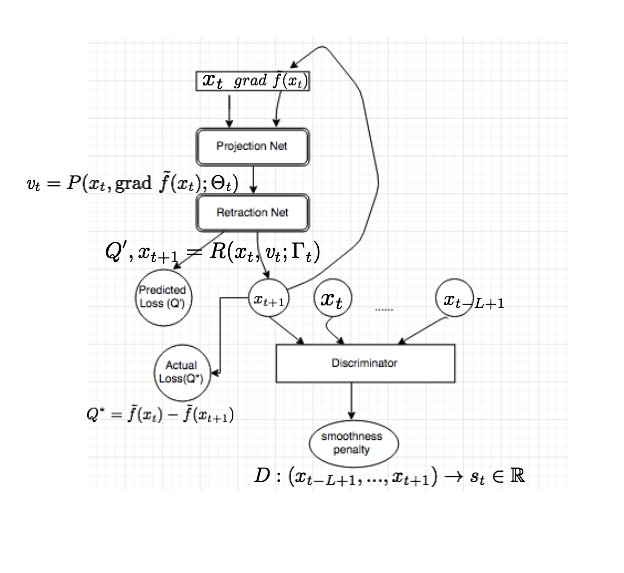
\includegraphics[width=8cm]
      {model.png}}
      \caption{\label{fig:my-label} one recurrency step of our framework}
\end{figure}




\end{document}
